\documentclass{project}
\usepackage[pdfauthor={Oscar Pocock, Kain Bryan-Jones},pdftitle={Software Engineering Group Project 20, User Interface Specification},pdftex]{hyperref}
\usepackage{float}
\usepackage{graphicx}
\graphicspath{ {./img/} } 
\newcommand*{\icon}[1]{%
  \raisebox{-.3\baselineskip}{%
    \includegraphics[
      height=\baselineskip,
      width=\baselineskip,
      keepaspectratio,
    ]{#1}%
  }%
}
\begin{document}
\title{Software Engineering Group Project 20}
\subtitle{User Interface Specification}
\author{Oscar Pocock, Kain Bryan-Jones}     
\shorttitle{Software Engineering Group Project 20 - User Interface Specification}
\version{0.4}
\status{For review}
\date{2020-02-20}
\configref{UISpecGroup20}
\maketitle
\tableofcontents
\newpage
\section{INTRODUCTION}
\subsection{Purpose of this Document}
The purpose of this document is to describe the user interface of the Welsh Vocabulary Tutor program which adheres to the User Interface Specifications Document\cite{se.qa.04} and General Documentation Standards\cite{se.qa.02} supplied by the client.

\subsection{Scope}
This document covers a descriptive representation of what the final user interface will look like, including how the product itself will be interacted with.\footnote{For the visual representation see the accompanied presentation document which demonstrates the use-cases of the program with mock-up screens of the UI.}

This document should be read by all project members. It is assumed that the reader is already familiar with the Welsh Vocabulary Tutor Requirements Specification\cite{se.qa.csrs}.
\subsection{Objectives}
The objectives of the document are:
\begin{itemize}
	\item To identify the typical users of the system
	\item To understand the individual use cases of users
	\item To predict the errors users may run into
	\item To describe how the errors will be handled
\end{itemize}

\section{TYPICAL USERS}
As described in Welsh Vocabulary Tutor Requirements Specification \emph{(Section 2.3)}\cite{se.qa.02} the program will be used by Welsh learners who are assumed to be experienced computer users. As this program is fairly basic in function and doesn't require authentication we assume that all users will have access to the same features but may use the program differently.
\subsection{Welsh Teacher}
Although they're less likely to use the program, the Welsh Teacher can use the program to easily create a dictionary and add vocabulary for their students to load in their version of the program to the study from.
\subsection{Welsh Learner}
The Welsh learner is an English speaker learning Welsh. They're using the program to help them memorise Welsh vocabulary as they find using a program easier than trying to memorise in other ways due to their competency with computers.
\subsubsection{Young Welsh Student}
The young Welsh students are less likely to add their own words and a more likely to be given a dictionary file to revise from by their teacher.
\subsubsection{Adult Welsh Learner}
The adult Welsh learner is likely to be independently learning the language and therefore is more likely to add their own vocabulary which fits their lifestyle or career.

\section{USE CASES}
This section highlights and describes the use cases of each user.
\\
\\
\textbf{Key}: [\textit{Use Case Reference}] - [\textit{Use Case Name}]
\subsection{Welsh Teacher}
\begin{itemize}
	\item 1 - View dictionary
	\item 7 - Load a new dictionary
	\item 8 - Add a new word
\end{itemize}

\subsection{Welsh Learners}
\subsubsection{Young Welsh Student}
\begin{itemize}
	\item 1 - View dictionary 
	\item 2 - Search for a word
	\item 3 - View practise list
	\item 4 - Modify the practise list
	\item 5 - Start a test
	\item 6 - View flashcards
	\item 7 - Load a new dictionary
	\item 9 - Change word ordering
\end{itemize}

\subsubsection{Adult Welsh Learner}
\begin{itemize}
	\item 1 - View dictionary
	\item 2 - Search for a word
	\item 3 - View practise list
	\item 4 - Modify the practise list
	\item 5 - Start a test
	\item 6 - View flashcards
	\item 7 - Load a new dictionary
	\item 8 - Add a new word
	\item 9 - Change word ordering
\end{itemize}
\begin{figure}[h]
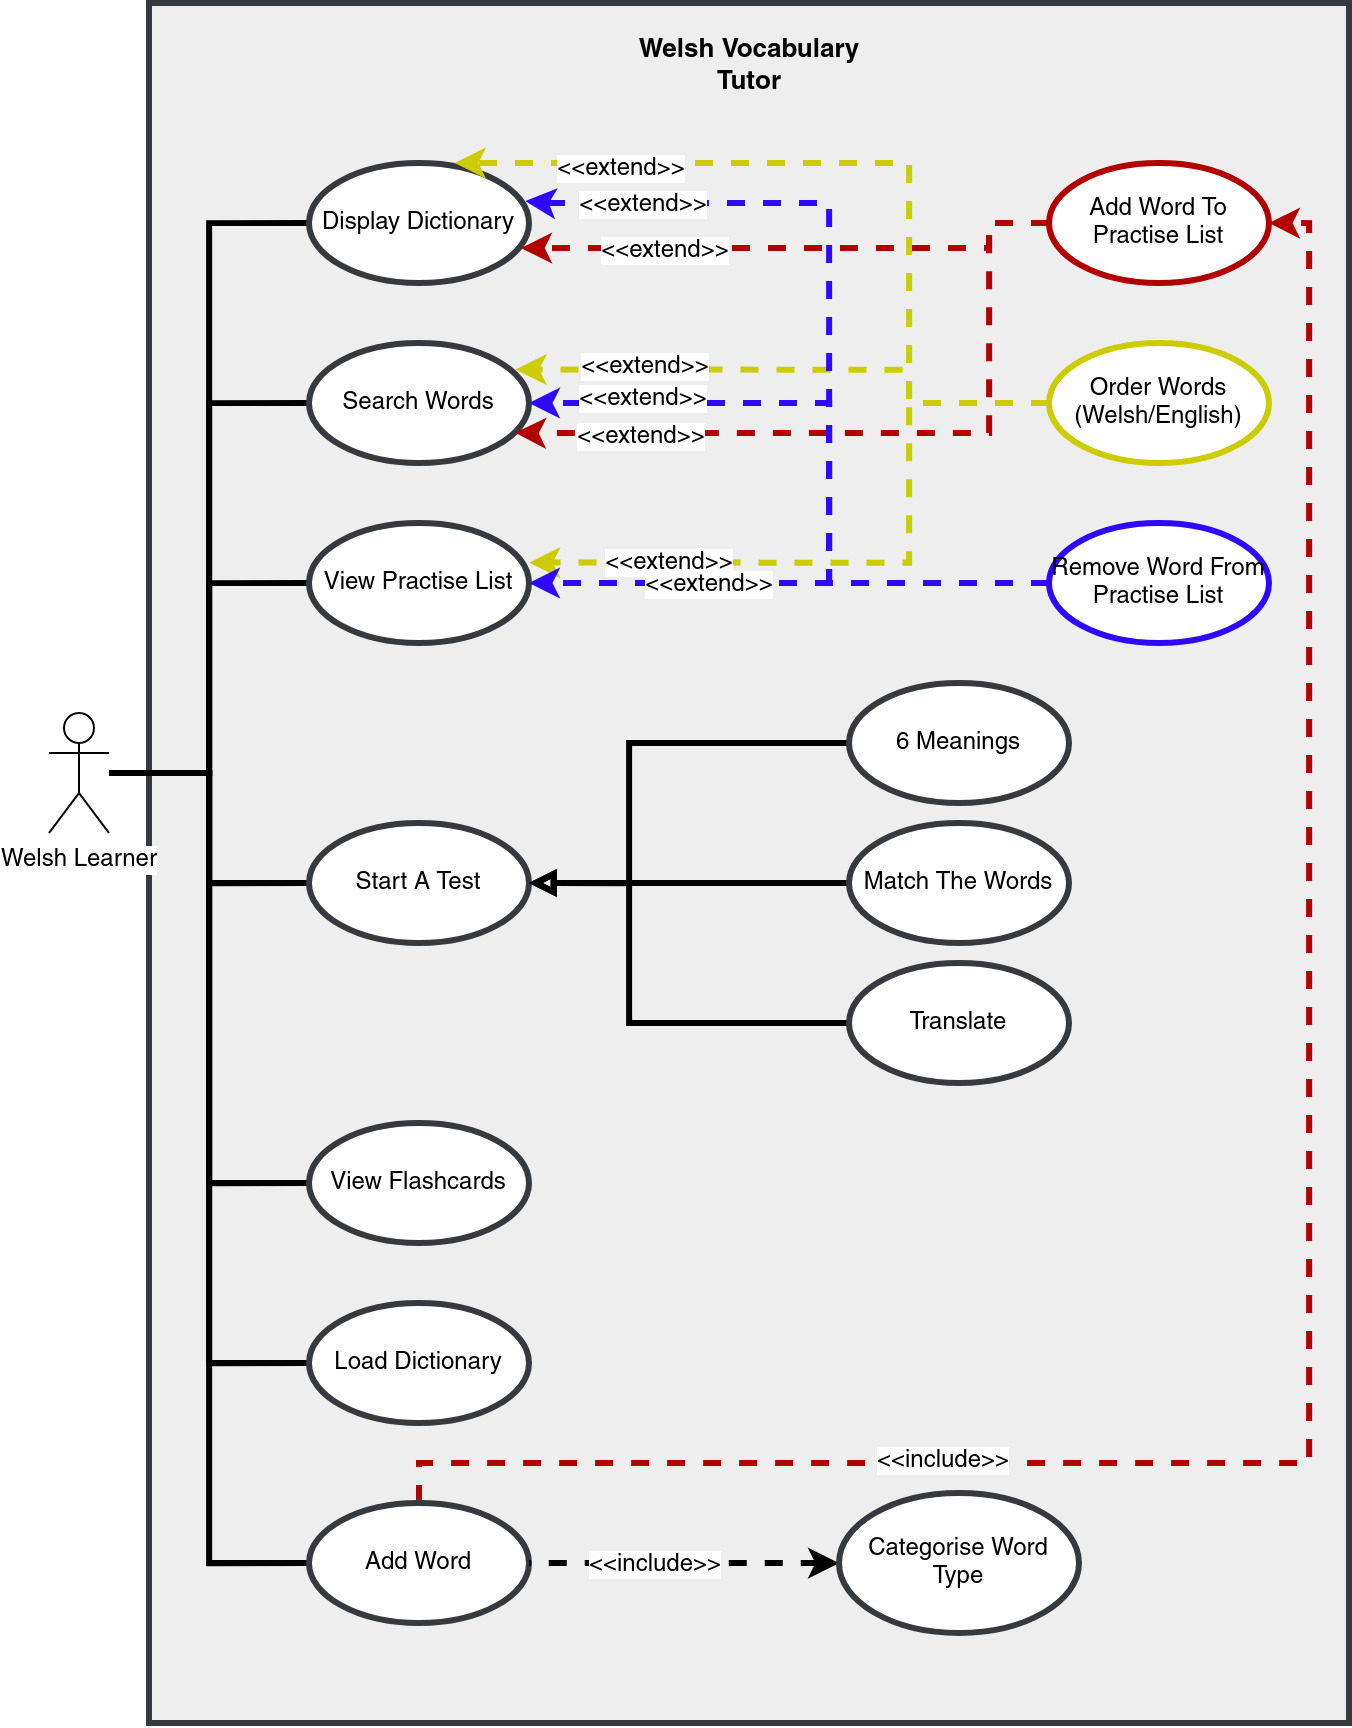
\includegraphics[width=\textwidth]{UCD}
\centering
	\caption{UML Use Case diagram of the Welsh Learner Group Class}
        \label{figure:1}
\end{figure}
\clearpage
\subsection{Use Case Descriptions}
\textbf{Use Case 1 View dictionary}
\\
When a user wants to view the dictionary they must first click the 'Dictionary \icon{dictionary-icon}' option from the main menu\footnote{This might not be necessary, as the startup page is the Dictionary page.}. The user is then presented with a view of all the words stored in the loaded dictionary file, English words on the left and their Welsh equivalent on the right. English verbs will have 'to' before the word, feminine Welsh nouns will have '\{f\}' after the word, and masculine Welsh nouns will have '\{m\}' after the word. If a word has multiple meanings in the other language the words will be displayed in a list next to it. The user will have the option to mark or unmark certain words for the practice list by clicking on a word. Words marked as practise words will be highlighted. A button marked as \icon{order-icon} and \icon{AZ-icon}/\icon{ZA-icon} gives the user the ability to change the ordering of the words (see use case 9). They also have the ability to search for words (see use case 2).
\\\\
\textbf{Use Case 2 Search for a word}
\\
When a user wants to search for a word they must first navigate to either the 'Dictionary \icon{dictionary-icon}' (see use case 1) or 'Practise List \icon{practise-icon}' (see use case 3) pages. Then they should click the text box next to the 'Search:' text. When the user types in the box it starts to filter words in the dictionary only displaying the words that begin with the string of characters written in the text box. The words that match are based on which language ordering is currently selected. If it is ordered by English the string in the text box will match the beginning of the English words, when switched to order by Welsh the search string will match the start of the Welsh words. If the word is not present then no results will appear for that search. All the searches are live or in other words refreshed per character typed in the search text box.
\\\\
\textbf{Use Case 3 View practise list}
\\
When a user wants to view the practise list they must first click on the 'Practise List \icon{practise-icon}' option from the menu. The user is then presented with a view of all the words they have marked as practise words, English words on the left and their Welsh equivalent on the right. English verbs will have 'to' before the word, feminine Welsh nouns will have '\{f\}' after the word, and masculine Welsh nouns will have '\{m\}' after the word. If a word has multiple meanings in the other language the words will be displayed in a list next to it. The user will have the option to remove certain words from the practise list by clicking on a word. A button marked as \icon{order-icon} and \icon{AZ-icon}/\icon{ZA-icon} gives the user the ability to change the ordering of the words (see use case 9). They also have the ability to search for words (see use case 2).
\\\\
\textbf{Use Case 4 Modify the practise list}
\\
When a user wants to modify the practise list they must first navigate to the 'Practise List \icon{practise-icon}' (see use case 3). Here the user can remove the words from the list if they so wish by clicking on the words. Note that adding a word from the dictionary to the practice list does not remove the word from the dictionary.
\\\\
\textbf{Use Case 5 Start a test}
\\
When a user wants to start a test they must first click on the 'Study \icon{study-icon}' option from the menu. They are then presented with three boxes denoting the different kind of tests\footnote{See Welsh Vocabulary Tutor Requirements Specification\cite{se.qa.csrs} \textit{(Section 3.1, FR9)}} which they can click on to take them to the selected test page (see use case 5.1, 5.2, and 5.3).
\\\\
\textbf{Use Case 5.1 Start 'Match The Meaning' test}
\\
When a user wants to start a 'Match The Word' test they must first navigate to the 'Study \icon{study-icon}' page (see use case 5 on how to navigate there) and then click the 'Match The Meaning' box. The user is then presented with eight words (four pairs), half of which are in English and half of which are the Welsh counterparts. It is the user's job to match the correct translations by ordering the words so that the correct pairs are presented side by side. On the top right of the page it shows the user how many right and wrong answers they have in that specific test.
\\\\
\textbf{Use Case 5.2 Start '6 Meanings' test}
\\
When a user wants to start a '6 Meanings' test they must first navigate to the 'Study \icon{study-icon}' page (see use case 5 on how to navigate there) and then click the '6 Meanings' box. The user is then presented with a large word in either Welsh or English and a bundle of words in the opposite language. It's the users job to click the word that matches the large word. On the top right of the page it shows the user how many right and wrong answers they have in that specific test.
\\\\
\textbf{Use Case 5.3 Start 'Translation ' test}
\\
When a user wants to start a 'Translation' test they must first navigate to the 'Study \icon{study-icon}' page (see use case 5 on how to navigate there) and then click the 'Translation' box. The user is then presented with a large word in either Welsh or English and a text box in which they need to type in the translation. On the top right of the page it shows the user how many right and wrong answers they have in that specific test.
\\\\
\textbf{Use Case 6 View flashcards}
\\
When a user wants to view flashcards they must first click on the 'Flashcards \icon{flashcard-icon}' option from the menu. The user is then presented with a flashcard in the centre of the screen. One side of the card has a word from their practise list and the other side has the translation of it. The user can flip the card by clicking on it and thus revealing the translation. If the user wishes to change to a different card they can do so by clicking the \icon{left-icon} and \icon{right-icon} to go to the previous or next card respectively. This page also shows them which card number they are on between the arrows and how many cards are available.
\\\\
\textbf{Use Case 7 Load a new dictionary}
\\
When a user wants to load in a new dictionary they must first click on the 'Load \icon{load-icon}' option from the menu. The user is then presented with a file manager pop up allowing them to select the file they want to load in from their filesystem. The words from the file are then loaded into the program replacing the old ones. The dictionaries are stored as JSON files and is therefore the only format allowed to be loaded.
\\\\
\textbf{Use Case 8 Add a new word}
\\
When a user wants to add a new word to the dictionary they must first click on the 'Add \icon{add-icon}' option from the menu. The user is then presented with a page with two text boxes, one for the English translation and one for the Welsh translation, a drop down box to specify the word type, buttons to add accents for Welsh words, and an 'Add Word' button. All fields must be filled before the user is allowed to click the 'Add Word' button. Once this button is clicked the word is added to the currently loaded dictionary and the practise list.
\\\\
\textbf{Use Case 9 Change word ordering}
\\
When a user wants to change the ordering of the word list from English to Welsh or vice versa (both ordered alphabetically) they must first be in the 'Dictionary \icon{dictionary-icon}' (see use case 1 on how to navigate there) or 'Practise List \icon{practise-icon}' (see use case 3 on how to navigate there) page. The user is then presented with the \icon{order-icon} icon and the words ordered in English by default. Once clicked, the words will then be ordered in Welsh. If the user wishes, they may switch the order back to English by pressing the \icon{order-icon} icon again. Similarly, if the user wishes to change the ordering from ascending to descending they can click on the \icon{AZ-icon}. Once clicked, this icon will change to \icon{ZA-icon} to show the user what ordering is currently active.
\\

\section{ERROR CONDITIONS}
Each error message prompt should let the user know what has gone wrong and what they need to do to resolve the issue.
\subsection{No Dictionary Loaded}
If the user hasn't uploaded a dictionary i.e. there are no words loaded, the program should prompt an error when trying to:
\begin{itemize}
	\item 1 - View dictionary
	\item 2 - Search for a word
	\item 3 - View practise list
	\item 4 - Modify the practise list
	\item 5 - Start a test
	\item 6 - View flashcards
	\item 9 - Change word ordering
\end{itemize}
The error should state:
\begin{center}
	\emph{'Warning: No dictionary loaded. Please load a dictionary or add a word before moving on.'}
\end{center}
This should prompt the user to either load a dictionary file or add a word.
\subsection{Dictionary Formatting Invalid}
The dictionary file should be a JSON file following strict formatting \emph{(SE.QA.CSRS Section 3.4, DC3)}\cite{se.qa.csrs} . If a user attempts to upload a JSON file with incorrect formatting the program should prompt an error when trying to:
\begin{itemize}
	\item 7 - Load Dictionary
\end{itemize}
The error should state:
\begin{center}
	\emph{'Warning: Invalid dictionary format. Please upload a dictionary with correct formatting.'}
\end{center}
This should prompt the user to load a dictionary file with correct formatting.
\subsection{No Practise Words}
If the user hasn't added any words to the practise list, the program should prompt an error when trying to:
\begin{itemize}
	\item 3 - View practise list
	\item 5 - Start a test
	\item 6 - View Flashcards
	\end{itemize}
The error should state:
\begin{center}
	\emph{'Warning: No practise words present. Please mark at least one word as a practise word.'}
\end{center}
This should prompt the user to add a word to the practise list.
\subsection{Not Defining Word Type When Adding A Word}
If the user hasn't defined the word type, the program should prompt an error when trying to:
\begin{itemize}
	\item 8 - Add a new word
	\end{itemize}
The error should state:
\begin{center}
	\emph{'Warning: Word type not defined. Please specify the word type.'}
\end{center}
This should prompt the user to select a word type from the drop down menu.
\subsection{One Or More Word Fields Not Filled When Adding A Word}
If the user hasn't defined the Welsh and English word for a new word, the program should prompt an error when trying to:
\begin{itemize}
	\item 8 - Add a new word
	\end{itemize}
The error should state:
\begin{center}
	\emph{'Warning: One or more word translation(s) are not defined. Please fill all text boxes.'}
\end{center}
This should prompt the user to type in the Welsh and English equivalent words in their associated text boxes.
\subsection{Adding a word pair that already exists}
If the user attempts to add a word pair that already exists, the program should prompt an error when trying to:
\begin{itemize}
	\item 8 - Add a new word
	\end{itemize}
The error should state:
\begin{center}
	\emph{'Warning: Word pair already exists. Please enter a new word pair.'}
\end{center}
This should prompt the user to type in a new unseen Welsh-English word pair.
\subsection{Starting 'Match The Meaning' With Less Than 4 Words In The Practise List}
If the user attempts to play the 'Match The Meaning' with less than 4 words in their practise list, the program should prompt an error when trying to:
\begin{itemize}
	\item 5.1 - Start 'Match The Meaning' test.
	\end{itemize}
The error should state:
\begin{center}
	\emph{'Warning: Less than 4 words present in the practise list. Please add at least 4 words to practise list to play "Match The Meaning".'}
\end{center}
This should prompt the user to add at least 4 words to the practise list.
\addcontentsline{toc}{section}{REFERENCES}
\begin{thebibliography}{5}
\bibitem{se.qa.02} \emph{Software Engineering Group Projects}
General Documentation Standards.
C. J. Price, N. W. Hardy, B.P. Tiddeman, SE.QA.02. 2.3 Release.
\bibitem{se.qa.04} \emph{Software Engineering Group Projects}
User Interface Specification Standards.
C. J. Price, N. W. Hardy, B.P. Tiddeman, SE.QA.04. 1.2 Release.
\bibitem{se.qa.csrs} \emph{Software Engineering Group Projects}
Welsh Vocabulary Tutor Requirements Specification.
C. J. Price, N. W. Hardy, B.P. Tiddeman, SE.QA.CSRC. 1.1 Release.
\end{thebibliography}
\addcontentsline{toc}{section}{DOCUMENT HISTORY}
\section*{DOCUMENT HISTORY}
\begin{tabular}{|l | l | l | l | l |}
\hline
Version & CCF No. & Date & Changes made to Document & Changed by \\
\hline
0.1 & N/A & 2020-02-15 & Initial creation & OP \\
\hline
0.2 & N/A & 2020-02-18 & Spell checks, formatting, and added icons & OP \\
\hline
0.3 & N/A & 2020-02-20 & Grammatical corrections, word sort use case, startup & OP \\
\hline
0.4 & N/A & 2020-02-23 & Correct grammar, edits to use case 1, 8, and 9 & OP \\
\hline
\end{tabular}
\label{thelastpage}
\end{document}
